\chapter{UML Use Case Diagram} \label{ch:procedure}

\begin{figure}[H]
    \centering
    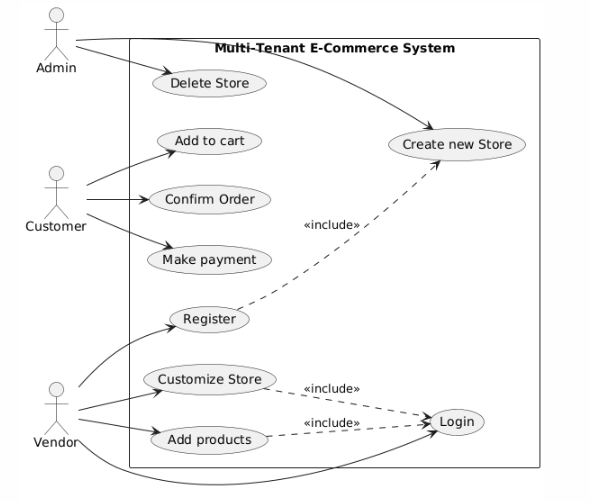
\includegraphics[width=1\linewidth]{figures/common use case uml.png}
    \caption{Multi-Tenant E-Commerce System Project UML Use case diagram}
    \label{fig:placeholder}
\end{figure}


\subsubsection*{Description}

This use case diagram provides a bird's-eye view of the entire Multi-Tenant E-Commerce System, illustrating the primary actors and their core interactions with the system. The diagram identifies three key actors: \textbf{Admin}, \textbf{Vendor}, and \textbf{Customer}.

\begin{itemize}
    \item \textbf{Admin:} The system administrator is responsible for overarching governance. The diagram shows the Admin actor connected to two key use cases: \textit{Delete Store} (to remove inappropriate or inactive vendor stores) and \textit{Login} (to access the admin panel). This actor represents the platform owner's operational control.
    
    \item \textbf{Vendor:} The small business owner (tenant) is the central user of the system. The diagram depicts the Vendor's core responsibilities, which include: \textit{Register} (to create their tenant account), \textit{Login} (to access their dashboard), \textit{Add Products} (to populate their inventory), and \textit{Customize Store} (to personalize their storefront's look and feel).
    
    \item \textbf{Customer:} The end-user who purchases products. The diagram shows the Customer's essential shopping journey: \textit{Register} (to create an account), \textit{Login} (to access their profile), \textit{Add to Cart} (to select items), \textit{Confirm Order} (to review and place the order), and \textit{Make Payment} (to complete the transaction).
\end{itemize}

This high-level diagram effectively communicates the system's boundaries and the distinct roles of each user type, serving as an excellent starting point for stakeholder discussions and scope validation.

\section*{Extended Use Cases}

\section{Diagram 1}

\subsection*{Use Case 1: Vendor Registration \& Subscription (FR-01)}

\textbf{Use Case Name:} Vendor Onboarding and Subscription Enforcement

\textbf{Primary Actor:} Prospective Vendor

\textbf{Secondary Actor:} Payment Gateway (e.g., bKash/Nagad)

\textbf{Goal:} To legally verify a new business, collect the subscription fee, and create a new tenant account.

\textbf{Preconditions:}
\begin{enumerate}
    \item The user possesses digital copies of their legal business documents.
\end{enumerate}

\textbf{Main Success Scenario:}
\begin{enumerate}
    \item The Prospective Vendor navigates to the registration page and inputs mandatory fields: Full Name, Business Email, Phone Number, Physical Address, Shop Type (Category), and a strong Password.
    
    \item \texttt{\textless\textless include\textgreater\textgreater} The system provides an interface for the applicant to upload digital copies of mandatory legal documents: E-TIN Certificate, Trade License/Certificate, and E-Return Submission Proof.
    
    \item The system validates the input format and enables the submission button.
    
    \item Upon successful data entry and document upload, the system redirects the user to a payment gateway.
    
    \item The vendor successfully completes the subscription payment.
    
    \item The system finalizes the account creation process and redirects the user to the "Registration Successful" page.
\end{enumerate}

\textbf{Extensions (Alternative Flows):}
\begin{enumerate}
    \item[2a.] \textbf{Missing Fields:} If any mandatory fields or documents are missing, the "Sign Up" button is disabled.
    
    \item[4a.] \texttt{\textless\textless extend\textgreater\textgreater} \textbf{Payment Failure:} If the payment fails, the user is returned to the payment screen with an error message. The account remains in a "Pending" state until the subscription is active.
\end{enumerate}

\textbf{Post Condition:}
\begin{enumerate}
    \item \textbf{Successful registration:} New tenant account is created with active subscription; vendor can access their store dashboard.
    \item \textbf{Pending registration:} Account created but marked as "Pending" until payment is successfully completed.
    \item \textbf{Failed registration:} No account created; vendor remains on registration page to correct errors.
\end{enumerate}


\subsection*{Use Case 2: Secure Login with 2FA (FR-01)}

\textbf{Use Case Name:} Secure Vendor Authentication

\textbf{Primary Actor:} Registered Vendor

\textbf{Goal:} To securely authenticate the vendor and prevent unauthorized access to financial and order history data.

\textbf{Preconditions:}
\begin{enumerate}
    \item The vendor has an active, fully registered account.
\end{enumerate}

\textbf{Main Success Scenario:}
\begin{enumerate}
    \item The Vendor enters their registered username and password on the login page.
    
    \item The system verifies the credentials.
    
    \item The system displays a "Verify OTP" screen.
    
    \item \texttt{\textless\textless include\textgreater\textgreater} The system sends a One-Time Password (OTP) to the vendor's registered email or phone number within 10 seconds.
    
    \item The Vendor enters the received OTP.
    
    \item The system verifies that the entered OTP matches the generated code.
    
    \item The system grants access to the vendor's dashboard.
\end{enumerate}

\textbf{Extensions (Alternative Flows):}
\begin{enumerate}
    \item[2a.] \textbf{Invalid Credentials:} If username or password is incorrect, system displays error message and remains on login page.
    
    \item[4a.] \textbf{OTP Delivery Failure:} If OTP cannot be delivered, system provides option to resend OTP or contact support.
    
    \item[6a.] \textbf{Invalid OTP:} Access is denied if the entered OTP does not match the generated code. System displays error message and allows OTP re-entry up to 3 attempts.
    
    \item[6b.] \textbf{OTP Expired:} If OTP is not entered within the validity period (e.g., 5 minutes), system displays "OTP Expired" and prompts to request a new OTP.
\end{enumerate}

\textbf{Post Condition:}
\begin{enumerate}
    \item \textbf{Successful authentication:} Vendor is granted access to their dashboard with a secure session.
    \item \textbf{Failed authentication:} Vendor remains on login/OTP screen; access is denied; failed attempts are logged for security monitoring.
\end{enumerate}


\subsection*{Use Case 3: Database Provisioning \& Data Routing (FR-02)}

\textbf{Use Case Name:} Automated Database Provisioning and Data Isolation

\textbf{Primary Actor:} System (Super Admin)

\textbf{Goal:} To automatically isolate tenant data and ensure queries are securely routed only to the correct vendor's database.

\textbf{Preconditions:}
\begin{enumerate}
    \item A new vendor has just successfully completed registration and their account is approved.
\end{enumerate}

\textbf{Main Success Scenario:}
\begin{enumerate}
    \item The System detects a newly approved vendor registration.
    
    \item \texttt{\textless\textless include\textgreater\textgreater} The System stores the vendor's global information, including Vendor Login Credentials, Subscription Status, and Tenant Metadata (Name, Shop URL), in the Central Database (Catalog DB).
    
    \item The System automatically provisions a distinct, isolated database dedicated solely to that vendor.
    
    \item The System initializes the new database with standard tables (Products, Orders, Customers) containing zero data.
    
    \item When the vendor makes a subsequent request (e.g., viewing "All Orders"), the System middleware identifies the incoming request's origin via the Tenant ID.
    
    \item The System dynamically routes the query to the correct isolated database, returning only their private business data.
\end{enumerate}

\textbf{Extensions (Alternative Flows):}
\begin{enumerate}
    \item[2a.] \textbf{Metadata Storage Failure:} If storing vendor information in Central Database fails, the system logs the error and notifies the Super Admin. Vendor account creation is rolled back.
    
    \item[3a.] \textbf{Database Provisioning Failure:} If automatic database creation fails, the system retries up to 3 times. After repeated failures, the system flags the vendor account for manual intervention and notifies the Super Admin.
    
    \item[5a.] \textbf{Attempted Data Breach:} If a query attempts to access another vendor's data (Cross-tenant SQL query), the system strictly prohibits it at the application level to ensure Vendor A cannot access Vendor B's data. The attempted breach is logged for security audit.
    
    \item[5b.] \textbf{Invalid Tenant ID:} If the Tenant ID is missing or invalid, the system rejects the request and returns an authentication error.
\end{enumerate}

\textbf{Post Condition:}
\begin{enumerate}
    \item \textbf{Successful provisioning:} New vendor has a dedicated, isolated database; all subsequent queries are correctly routed to the appropriate tenant database; data isolation is maintained.
    \item \textbf{Failed provisioning:} Vendor account is flagged; Super Admin is notified; manual intervention may be required to complete the provisioning process.
    \item \textbf{Security violation:} Any cross-tenant access attempts are blocked and logged; data integrity and isolation are preserved.
\end{enumerate}

\begin{figure}[H]
    \centering
    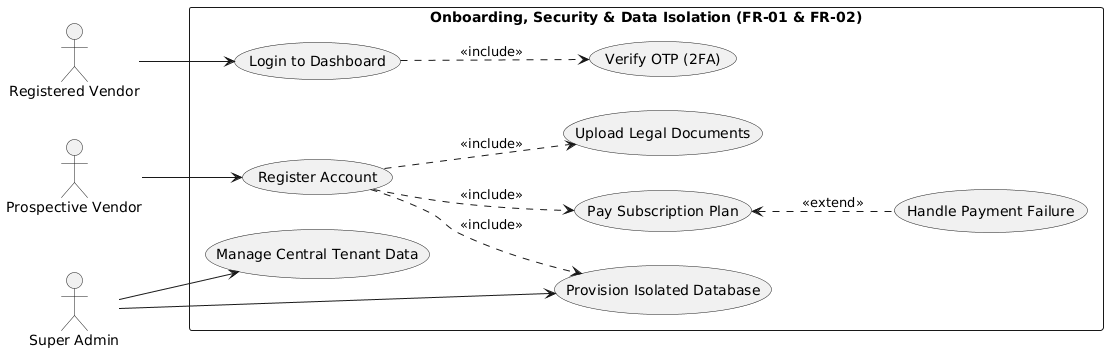
\includegraphics[width=1\linewidth]{dg01.png}
    \caption{Onboarding, security and data isolation}
    \label{fig:placeholder}
\end{figure}

\section{Diagram 2: Vendor-Specific Use Case Diagram (Offers \& Store Customization)}

\subsection{Use Case Scenario 3: Create Percentage Discount with Deadline}

\textbf{Use Case Name:} Create Percentage Discount with Deadline

\textbf{Actor:} Vendor

\textbf{Scenario / Description:}
\begin{enumerate}
    \item Vendor logs into their store dashboard.
    \item Vendor navigates to "Offers \& Promotions" section.
    \item Vendor selects "Create New Offer" and chooses "Percentage Discount."
    \item Vendor enters discount details:
    \begin{enumerate}
        \item Discount percentage (e.g., 10\%, 20\%, 50\%)
        \item Products or categories to apply discount to
        \item Minimum purchase amount (if applicable)
    \end{enumerate}
    \item System enforces \texttt{\textless\textless include\textgreater\textgreater} relationship: Vendor must set an offer deadline.
    \item Vendor selects offer start date and end date (deadline).
    \item System validates that end date is after start date and not in the past.
    \item Vendor optionally sets a coupon limit (maximum number of redemptions).
    \item Vendor reviews and confirms the discount offer details.
    \item System saves the discount offer and activates it according to the schedule.
    \item System displays the new offer in the vendor's active promotions list.
\end{enumerate}

\textbf{Exception:}
\begin{enumerate}
    \item Deadline (end date) is not set (violates mandatory \texttt{\textless\textless include\textgreater\textgreater} requirement).
    \item End date is earlier than start date.
    \item Start date or end date is in the past.
    \item Discount percentage is invalid (e.g., negative, zero, or >100\%).
    \item No products or categories selected for the discount.
    \item Coupon limit is set to an invalid value (negative or zero when required).
    \item Database connection failure during offer creation.
\end{enumerate}

\textbf{Precondition:}
\begin{enumerate}
    \item Vendor is logged into the system with valid session.
    \item Vendor has products listed in their inventory.
    \item System database is operational.
\end{enumerate}

\textbf{Post Condition:}
\begin{enumerate}
    \item \textbf{Successful discount creation:} New percentage discount offer is created and saved in the system; offer is scheduled according to start/end dates; customers can now avail the discount on eligible products; offer appears in vendor's promotions list.
    \item \textbf{Unsuccessful discount creation:} Discount offer is not saved; system displays appropriate error messages (e.g., "Deadline must be set," "End date must be after start date"); vendor remains on offer creation page to correct errors.
    \item \textbf{Exception:} Transaction is rolled back; system displays error message; vendor remains on offer creation page if possible.
\end{enumerate}

\begin{figure}[H]
    \centering
    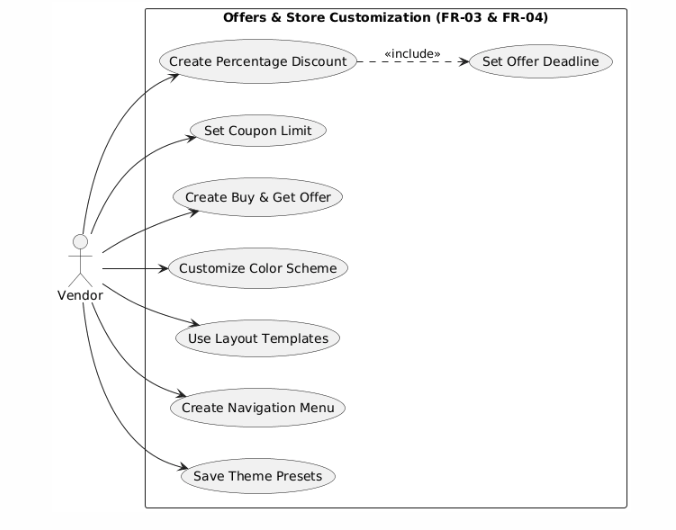
\includegraphics[width=1\linewidth]{figures/Extended usecase.png}
    \caption{Vendor specific customization and discount offers' UML Use case diagram}
    \label{fig:placeholder}
\end{figure}


\section{Extended Use Cases: Payment \& Delivery Management}

%-----------------------------------------------------------------------------
% Use Case 1: Multi-Method Payment Processing
%-----------------------------------------------------------------------------
\subsection*{Use Case 1: Multi-Method Payment Processing (FR-05)}

\textbf{Use Case Name:} Process Order Payment

\textbf{Primary Actor:} Customer

\textbf{Secondary Actor:} System, Payment Gateway (External)

\textbf{Goal:} To allow customers to pay for orders using multiple online payment gateways or Cash on Delivery (COD).

\textbf{Preconditions:}
\begin{enumerate}
    \item The Customer has items in the shopping cart.
    \item The Customer is logged into the system.
\end{enumerate}

\textbf{Main Success Scenario:}
\begin{enumerate}
    \item The Customer proceeds to checkout.
    \item The Customer selects a preferred payment method (online or COD).
    \item If an online payment is selected, the system redirects the Customer to the chosen payment gateway.
    \item The Customer completes payment through the gateway.
    \item The system verifies the payment status.
    \item The system updates the order status as "Paid" or "Failed".
    \item If COD is selected, the system marks payment status as "Pending (COD)".
    \item The system confirms the order and stores payment details.
\end{enumerate}

\textbf{Extensions (Alternative Flows):}
\begin{enumerate}
    \item[3a.] \textbf{Payment Failure:} If the online payment fails, the system cancels order confirmation and displays an error message.
    \item[3b.] \textbf{Invalid Payment Method:} If the selected payment method is unavailable, the system prompts the Customer to choose a different method.
    \item[4a.] \texttt{\textless\textless extend\textgreater\textgreater} \textbf{Payment Gateway Timeout:} If the payment gateway does not respond within the specified time, the system cancels the transaction and notifies the customer to try again.
\end{enumerate}

\textbf{Post Condition:}
\begin{enumerate}
    \item \textbf{Successful payment:} Order is confirmed with status "Paid" (online) or "Pending (COD)"; payment details are stored.
    \item \textbf{Failed payment:} Order is not confirmed; customer remains on checkout page with error message.
\end{enumerate}


%-----------------------------------------------------------------------------
% Use Case 2: Payment Method Selection
%-----------------------------------------------------------------------------
\subsection*{Use Case 2: Payment Method Selection (FR-05)}

\textbf{Use Case Name:} Choose Payment Method

\textbf{Primary Actor:} Customer

\textbf{Secondary Actor:} System

\textbf{Goal:} To allow the Customer to select a preferred payment method during checkout.

\textbf{Preconditions:}
\begin{enumerate}
    \item The Customer has items in the shopping cart.
    \item The Customer is logged into the system.
\end{enumerate}

\textbf{Main Success Scenario:}
\begin{enumerate}
    \item The Customer navigates to the checkout page.
    \item The system displays all available payment options (bKash, Nagad, Visa, MasterCard, COD).
    \item The Customer selects a payment method.
    \item The system shows the selected method in the order summary.
    \item The Customer submits the order.
    \item The system confirms order creation based on the chosen payment method.
\end{enumerate}

\textbf{Extensions (Alternative Flows):}
\begin{enumerate}
    \item[2a.] \textbf{No Payment Methods Available:} If no payment methods are configured or available, the system displays an error message and prevents order submission.
    \item[3a.] \textbf{Method Unavailable:} If the selected payment method is temporarily unavailable, the system prompts the Customer to choose an alternative method.
    \item[5a.] \textbf{Order Submission Without Selection:} If the Customer attempts to submit the order without selecting a payment method, the system highlights the required field and prevents submission.
\end{enumerate}

\textbf{Post Condition:}
\begin{enumerate}
    \item \textbf{Successful selection:} Payment method is recorded with the order; order processing continues based on the selected method.
    \item \textbf{Unsuccessful selection:} Order is not submitted; customer remains on checkout page.
\end{enumerate}

\vspace{0.5cm}
\hrule
\vspace{0.5cm}

%-----------------------------------------------------------------------------
% Use Case 3: Online Payment Verification
%-----------------------------------------------------------------------------
\subsection*{Use Case 3: Online Payment Verification (FR-05)}

\textbf{Use Case Name:} Verify Online Payment

\textbf{Primary Actor:} Customer

\textbf{Secondary Actor:} System, Payment Gateway (External)

\textbf{Goal:} To ensure the Customer's online payment is successfully completed before confirming the order.

\textbf{Preconditions:}
\begin{enumerate}
    \item The Customer has selected an online payment method.
    \item The Customer has proceeded to the payment gateway.
\end{enumerate}

\textbf{Main Success Scenario:}
\begin{enumerate}
    \item The system redirects the Customer to the payment gateway.
    \item The Customer completes payment through the gateway interface.
    \item The system receives payment confirmation from the gateway (callback/webhook).
    \item If payment succeeds, the system marks the order as "Paid".
    \item If payment fails, the system shows an error and does not confirm the order.
    \item The system redirects the Customer back to the order confirmation or failure page.
\end{enumerate}

\textbf{Extensions:}
\begin{enumerate}
    \item[3a.] \textbf{Payment Timeout:} If the payment process times out, the system cancels the transaction and notifies the Customer to try again.
    \item[3b.] \textbf{Duplicate Payment:} If the same payment is processed twice, the system detects duplication and initiates refund for the duplicate transaction.
    \item[3c.] \textbf{Invalid Callback:} If the system receives an invalid or unverified callback from the gateway, it rejects the update and logs the incident for security review.
\end{enumerate}

\textbf{Post Condition:}
\begin{enumerate}
    \item \textbf{Payment successful:} Order status updated to "Paid"; customer receives confirmation; inventory is updated.
    \item \textbf{Payment failed:} Order remains in "Pending Payment" or is cancelled; customer is prompted to retry payment.
\end{enumerate}

\vspace{0.5cm}
\hrule
\vspace{0.5cm}

%-----------------------------------------------------------------------------
% Use Case 4: Product Delivery Tracking
%-----------------------------------------------------------------------------
\subsection*{Use Case 4: Product Delivery Tracking (FR-06)}

\textbf{Use Case Name:} Track Order Delivery

\textbf{Primary Actor:} Customer

\textbf{Secondary Actor:} System, Third-Party Courier API (Pathao, RedX, etc.)

\textbf{Goal:} To provide real-time tracking of order delivery via third-party courier services.

\textbf{Preconditions:}
\begin{enumerate}
    \item The Customer has placed an order.
    \item The order has been dispatched via a third-party courier.
    \item A valid tracking ID has been generated and associated with the order.
\end{enumerate}

\textbf{Main Success Scenario:}
\begin{enumerate}
    \item The Customer navigates to the order details page.
    \item The system fetches delivery status from courier APIs (Pathao, RedX, etc.) using the tracking ID.
    \item The system displays the current delivery status with timestamp (e.g., Picked Up, In Transit, Out for Delivery, Delivered).
    \item The delivery status updates automatically as the shipment progresses.
    \item Upon delivery completion, the system marks the order as "Delivered" and optionally requests feedback.
\end{enumerate}

\textbf{Extensions:}
\begin{enumerate}
    \item[2a.] \textbf{API Unavailable:} If the courier API is temporarily unavailable, the system displays the last known status and retries connection periodically.
    \item[2b.] \textbf{Invalid Tracking ID:} If the tracking ID is invalid or not found, the system displays a message asking the customer to contact support.
    \item[3a.] \textbf{Delivery Exception:} If the courier reports an exception (e.g., address not found, recipient unavailable), the system displays the exception details and suggests next steps.
\end{enumerate}

\textbf{Post Condition:}
\begin{enumerate}
    \item \textbf{Successful tracking:} Customer can view real-time delivery status; system maintains synchronization with courier updates.
    \item \textbf{Delivery completed:} Order status updated to "Delivered"; customer may be prompted to rate their experience.
\end{enumerate}

\vspace{0.5cm}
\hrule
\vspace{0.5cm}

%-----------------------------------------------------------------------------
% Use Case 5: Vendor Delivery Monitoring
%-----------------------------------------------------------------------------
\subsection*{Use Case 5: Vendor Delivery Monitoring (FR-06)}

\textbf{Use Case Name:} Monitor Shipment Status

\textbf{Primary Actor:} Vendor

\textbf{Secondary Actor:} System, Third-Party Courier API (Pathao, RedX, etc.)

\textbf{Goal:} To allow Vendors to monitor delivery status of customer orders in real-time.

\textbf{Preconditions:}
\begin{enumerate}
    \item The Vendor is logged into the system.
    \item Orders have been confirmed and dispatched with valid tracking IDs.
\end{enumerate}

\textbf{Main Success Scenario:}
\begin{enumerate}
    \item The Vendor navigates to their dashboard or "Orders" section.
    \item The system displays a list of all orders with their current status.
    \item For dispatched orders, the system retrieves courier-provided tracking information for each order via API integration.
    \item The Vendor views delivery progress for each order (Picked Up, In Transit, Delivered, Returned).
    \item The system automatically updates statuses as the courier updates the shipment.
    \item The Vendor can filter orders by delivery status to identify pending, delivered, or returned shipments.
\end{enumerate}

\textbf{Extensions:}
\begin{enumerate}
    \item[3a.] \textbf{Bulk Status Update:} The system periodically (e.g., every 30 minutes) batches API calls to update all active shipments efficiently.
    \item[3b.] \textbf{Delivery Exception Alert:} If a shipment encounters an exception (e.g., return to sender), the system highlights the order and optionally sends a notification to the Vendor.
    \item[4a.] \textbf{Manual Status Override:} In case of API failure, the Vendor may have the ability to manually update delivery status (with appropriate audit logging).
    \item[5a.] \textbf{Export Delivery Report:} The Vendor can export delivery data for reconciliation and accounting purposes.
\end{enumerate}

\textbf{Post Condition:}
\begin{enumerate}
    \item \textbf{Successful monitoring:} Vendor has up-to-date visibility of all shipment statuses; can take action on exceptions.
    \item \textbf{Delivery completed:} Orders marked as delivered are moved to completed orders; revenue can be reconciled.
    \item \textbf{Exception handling:} Returned or undelivered orders are flagged for Vendor action (e.g., customer contact, refund processing).
\end{enumerate}

\begin{figure}[H]
    \centering
    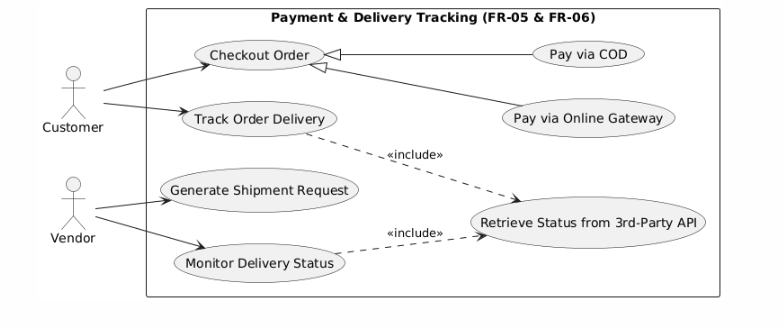
\includegraphics[width=1\linewidth]{figures/dg03.png}
    \caption{Payment \& Delivery Management}
    \label{fig:placeholder}
\end{figure}

\section{Extended Use Cases: Notifications \& Reviews Management}

%-----------------------------------------------------------------------------
% Use Case 1: Promotional Notification Management
%-----------------------------------------------------------------------------
\subsection*{Use Case 1: Promotional Notification Management (FR-09)}

\textbf{Use Case Name:} Send Promotional Notification

\textbf{Primary Actor:} Vendor

\textbf{Secondary Actor:} System, Notification Service (Email/SMS/Push)

\textbf{Goal:} To notify customers about promotions, offers, or announcements to increase engagement and sales.

\textbf{Preconditions:}
\begin{enumerate}
    \item The Vendor has an active account.
    \item The Vendor is logged into the dashboard.
    \item The system has customer contact information (email/phone) for selected audience.
\end{enumerate}

\textbf{Main Success Scenario:}
\begin{enumerate}
    \item The Vendor navigates to the promotional notifications section from the dashboard.
    \item The Vendor selects the option to create a new promotional notification.
    \item The Vendor enters the notification content (offer details, message text).
    \item \texttt{\textless\textless include\textgreater\textgreater} The system prompts the Vendor to select the target audience.
    \item The Vendor selects the desired customer group (all customers or a specific segment based on purchase history, location, etc.).
    \item The Vendor submits the promotional notification.
    \item The system sends the notification to the selected customers via configured channels (email, SMS, in-app notification).
    \item The system stores the notification details in the notification history for future reference.
\end{enumerate}

\textbf{Extensions (Alternative Flows):}
\begin{enumerate}
    \item[4a.] \textbf{No Customer Segments Available:} If no customer segments are defined, the system defaults to "All Customers" and notifies the Vendor.
    \item[5a.] \textbf{Empty Audience Selection:} If the Vendor selects a segment with zero customers, the system warns and prompts to select a different audience or cancel.
    \item[7a.] \textbf{Notification Delivery Failure:} If some notifications fail to send (e.g., invalid email/phone), the system logs failures and continues sending to remaining customers.
    \item[7b.] \texttt{\textless\textless extend\textgreater\textgreater} \textbf{Bulk Sending Rate Limit:} If sending to a large audience, the system implements rate limiting to avoid being flagged as spam.
\end{enumerate}

\textbf{Post Condition:}
\begin{enumerate}
    \item \textbf{Successful sending:} Promotional notifications are delivered to target customers; notification is recorded in history with timestamp and audience size.
    \item \textbf{Partial success:} Some notifications failed but were logged; Vendor can view delivery report in history.
    \item \textbf{Failure:} No notifications sent; Vendor remains on creation page with error message.
\end{enumerate}

\vspace{0.5cm}
\hrule
\vspace{0.5cm}

%-----------------------------------------------------------------------------
% Use Case 2: View Notification History
%-----------------------------------------------------------------------------
\subsection*{Use Case 2: View Notification History (FR-09)}

\textbf{Use Case Name:} View Notification History

\textbf{Primary Actor:} Vendor

\textbf{Secondary Actor:} System

\textbf{Goal:} To review previously sent promotional notifications for tracking and analysis.

\textbf{Preconditions:}
\begin{enumerate}
    \item The Vendor is logged into the system.
    \item Previous promotional notifications have been sent.
\end{enumerate}

\textbf{Main Success Scenario:}
\begin{enumerate}
    \item The Vendor navigates to the notification history section from the dashboard.
    \item The system retrieves all previously sent promotional notifications from the database.
    \item The system displays the notification list with the following details for each:
    \begin{enumerate}
        \item Date and time sent
        \item Notification title/message preview
        \item Target audience (e.g., "All Customers" or segment name)
        \item Delivery status (Sent, Failed, Partial)
        \item Open/click rate (if tracking is enabled)
    \end{enumerate}
    \item The Vendor can filter or search through the history by date range or message content.
    \item The Vendor selects a specific notification to view full details and delivery report.
\end{enumerate}

\textbf{Extensions (Alternative Flows):}
\begin{enumerate}
    \item[2a.] \textbf{No History Available:} If no notifications have been sent yet, the system displays a message "No notification history found" with a link to create a new notification.
    \item[3a.] \textbf{Analytics Unavailable:} If engagement tracking (opens/clicks) is not configured, the system displays "Tracking not available" for those fields.
    \item[5a.] \textbf{Export History:} The Vendor may have the option to export notification history as CSV/PDF for reporting purposes.
\end{enumerate}

\textbf{Post Condition:}
\begin{enumerate}
    \item \textbf{Successful view:} Vendor can review all past promotional communications; data can be used to analyze campaign effectiveness.
    \item \textbf{No data:} Vendor is informed that no notifications have been sent yet.
\end{enumerate}

\vspace{0.5cm}
\hrule
\vspace{0.5cm}

%-----------------------------------------------------------------------------
% Use Case 3: Customer Review & Rating Submission
%-----------------------------------------------------------------------------
\subsection*{Use Case 3: Customer Review \& Rating Submission (FR-10)}

\textbf{Use Case Name:} Submit Product Review and Rating

\textbf{Primary Actor:} Customer

\textbf{Secondary Actor:} System

\textbf{Goal:} To allow customers to submit feedback for purchased products, helping other customers make informed decisions.

\textbf{Preconditions:}
\begin{enumerate}
    \item The Customer has completed a purchase (order status: Delivered).
    \item The Customer is logged into the system.
    \item The product is still available in the system catalog.
\end{enumerate}

\textbf{Main Success Scenario:}
\begin{enumerate}
    \item The Customer navigates to the order history page.
    \item The Customer selects a purchased product from a delivered order to review.
    \item The Customer enters a rating (1–5 stars) and written feedback (optional but encouraged).
    \item \texttt{\textless\textless include\textgreater\textgreater} The system verifies that the product was actually purchased by the Customer (checks order history).
    \item The Customer submits the review.
    \item The system validates the input (rating range, content length).
    \item The system saves the review in the database and associates it with the product and customer.
    \item The system recalculates and updates the product's average rating based on all reviews.
    \item The review becomes visible on the product details page for all customers to see.
\end{enumerate}

\textbf{Extensions (Alternative Flows):}
\begin{enumerate}
    \item[2a.] \textbf{Already Reviewed:} If the Customer has already reviewed this product, the system displays "You have already reviewed this product" and allows editing instead of new submission.
    
    \item[4a.] \textbf{Purchase Not Verified:} If the product was not purchased by this Customer, the system denies the review submission and displays "You can only review products you have purchased."
    
    \item[6a.] \textbf{Invalid Rating:} If the rating is outside the allowed range (e.g., 0 or 6), the system displays an error message "Rating must be between 1 and 5 stars."
    
    \item[6b.] \textbf{Inappropriate Content:} If the review contains prohibited words/phrases, the system flags it for moderation or rejects with an appropriate message.
    
    \item[7a.] \textbf{Database Error:} If saving fails, the system displays an error and prompts the Customer to try again later.
\end{enumerate}

\textbf{Post Condition:}
\begin{enumerate}
    \item \textbf{Successful submission:} New review is live on the product page; product's average rating is updated; other customers can see the feedback.
    \item \textbf{Failed submission:} Review is not saved; Customer receives error message and can correct and resubmit.
    \item \textbf{Flagged review:} Review is saved but marked for moderation; not visible publicly until approved.
\end{enumerate}

\vspace{0.5cm}
\hrule
\vspace{0.5cm}

%-----------------------------------------------------------------------------
% Use Case 4: Flag Inappropriate Review
%-----------------------------------------------------------------------------
\subsection*{Use Case 4: Flag Inappropriate Review (FR-10)}

\textbf{Use Case Name:} Flag Inappropriate Review

\textbf{Primary Actor:} Vendor

\textbf{Secondary Actor:} System, Administrator (for final action)

\textbf{Goal:} To report inappropriate, fraudulent, or misleading customer reviews for moderation and potential removal.

\textbf{Preconditions:}
\begin{enumerate}
    \item The Vendor is logged into the system.
    \item A customer review exists for the Vendor's product.
    \item The Vendor has identified a review that violates platform guidelines.
\end{enumerate}

\textbf{Main Success Scenario:}
\begin{enumerate}
    \item The Vendor navigates to the product reviews section for one of their products.
    \item The Vendor browses through customer reviews and identifies an inappropriate review.
    \item The Vendor selects the review and clicks the "Flag" or "Report" option.
    \item The system prompts the Vendor to select a reason for flagging (e.g., Spam, False Information, Abusive Language, Off-topic).
    \item The Vendor optionally adds additional comments or context.
    \item The Vendor submits the flag request.
    \item The system marks the review as "Flagged" in the database and changes its status to "Under Review."
    \item The system sends a notification to the Administrator for manual moderation.
    \item The review is temporarily hidden from public view or remains visible pending review (based on platform policy).
\end{enumerate}

\textbf{Extensions (Alternative Flows):}
\begin{enumerate}
    \item[4a.] \textbf{No Reason Selected:} If the Vendor attempts to flag without selecting a reason, the system prompts "Please select a reason for flagging this review."
    
    \item[7a.] \textbf{Auto-Moderation:} Based on platform configuration, the system may automatically hide reviews flagged for certain reasons (e.g., hate speech) without admin intervention.
    
    \item[8a.] \textbf{Duplicate Flag:} If the same review has already been flagged by another Vendor/Customer, the system increments the flag count and notifies "This review has already been reported."
    
    \item[9a.] \textbf{Administrator Decision:} After review, the Administrator may:
    \begin{enumerate}
        \item Remove the review entirely if found inappropriate
        \item Restore the review if flagged in error
        \item Warn the Customer who posted the review
    \end{enumerate}
\end{enumerate}

\textbf{Post Condition:}
\begin{enumerate}
    \item \textbf{Successful flagging:} Review is marked "Under Review"; Administrator is notified; temporary action may be taken based on policy.
    \item \textbf{Review removed:} If Administrator confirms violation, review is permanently removed from product page.
    \item \textbf{Review restored:} If flagged in error, review is reinstated and flag is removed.
    \item \textbf{Vendor notified:} Vendor receives notification of the final decision on their flag request.
\end{enumerate}

\begin{figure}[H]
    \centering
    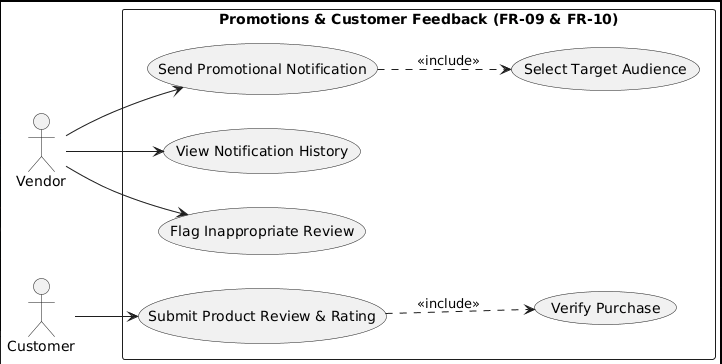
\includegraphics[width=1\linewidth]{figures/dg04.png}
    \caption{Promotions and customer feedback}
    \label{fig:placeholder}
\end{figure}

\section{Extended Use Cases: Inventory \& Analytics Management}

%-----------------------------------------------------------------------------
% Use Case 1: Manage Inventory
%-----------------------------------------------------------------------------
\subsection*{Use Case 1: Manage Inventory (FR-07)}

\textbf{Use Case Name:} Manage Inventory

\textbf{Primary Actor:} Vendor

\textbf{Secondary Actor:} System

\textbf{Goal:} To provide vendors full control over product lifecycle and maintain accurate stock levels.

\textbf{Preconditions:}
\begin{itemize}
    \item The Vendor has an active account and is logged into the system.
\end{itemize}

\textbf{Main Success Scenario:}
\begin{enumerate}
    \item The Vendor navigates to the Inventory Management section of the dashboard.
    \item The Vendor selects the option to add a new product.
    \item The Vendor inputs the product name, price, SKU, and initial quantity.
    \item The system validates the input and stores the product in the central database.
    \item The Vendor sets a "Low Stock" threshold for the product.
    \item The system confirms the product is live and synchronized with the digital storefront.
\end{enumerate}

\textbf{Extensions (Alternative Flows):}
\begin{itemize}
    \item[3a.] \textbf{Manual Stock Update:} The Vendor edits an existing product's quantity.
    \begin{itemize}
        \item \textbf{Validation:} The system implements rules to prevent stock quantities from falling below zero.
    \end{itemize}
    
    \item[3b.] \textbf{Remove Product:} The Vendor removes a product from the system, and the storefront reflects this change instantly.
    
    \item[4a.] \textbf{Invalid Input:} If the vendor enters invalid data (negative price, duplicate SKU, etc.), the system displays an error message and prevents submission.
    
    \item[5a.] \textbf{Threshold Validation:} If the low stock threshold is set higher than the initial quantity, the system warns the vendor but allows the setting.
\end{itemize}

\textbf{Post Condition:}
\begin{itemize}
    \item \textbf{Successful addition:} New product is live in the storefront with accurate initial stock.
    \item \textbf{Successful update:} Existing product stock levels are updated and reflected immediately.
    \item \textbf{Successful removal:} Product is no longer visible in the storefront.
    \item \textbf{Failed operation:} No changes are made; vendor receives appropriate error message.
\end{itemize}

\vspace{0.5cm}
\hrule
\vspace{0.5cm}

%-----------------------------------------------------------------------------
% Use Case 2: View Analytics Dashboard
%-----------------------------------------------------------------------------
\subsection*{Use Case 2: View Analytics Dashboard (FR-08)}

\textbf{Use Case Name:} View Analytics Dashboard

\textbf{Primary Actor:} Vendor

\textbf{Secondary Actor:} System

\textbf{Goal:} To translate raw sales data into actionable insights through visual charts.

\textbf{Preconditions:}
\begin{itemize}
    \item The Vendor is logged into the system and has existing sales data.
\end{itemize}

\textbf{Main Success Scenario:}
\begin{enumerate}
    \item The Vendor navigates to the Analytical Board from the main menu.
    \item The system retrieves real-time sales data from the database.
    \item The system calculates and displays Key Performance Indicators (KPIs) including total sales, revenue, and order counts.
    \item The system renders a ranked list of best-selling items.
    \item The system displays revenue trends using bar charts and product distribution using pie charts.
\end{enumerate}

\textbf{Extensions (Alternative Flows):}
\begin{itemize}
    \item[2a.] \textbf{No Data Available:} If the vendor has no sales data yet, the system displays a message "No sales data available" with suggestions to start promoting products.
    
    \item[3a.] \textbf{Data Calculation Delay:} If data volume is large, the system shows a loading indicator while calculating KPIs.
    
    \item[5a.] \textbf{Chart Rendering Error:} If charts fail to render, the system displays data in tabular format as fallback.
\end{itemize}

\textbf{Post Condition:}
\begin{itemize}
    \item \textbf{Successful view:} Vendor can see comprehensive sales analytics with visual representations.
    \item \textbf{No data:} Vendor is informed that no sales data exists yet.
\end{itemize}

\vspace{0.5cm}
\hrule
\vspace{0.5cm}

%-----------------------------------------------------------------------------
% Use Case 3: Filter Data by Date (FR-08 Extension)
%-----------------------------------------------------------------------------
\subsection*{Use Case 3: Filter Data by Date (FR-08 Extension)}

\textbf{Use Case Name:} Filter Data by Date

\textbf{Primary Actor:} Vendor

\textbf{Secondary Actor:} System

\textbf{Goal:} To refine dashboard visualizations and metrics by a user-defined timeframe.

\textbf{Relationship:} \texttt{\textless\textless extend\textgreater\textgreater} to View Analytics Dashboard

\textbf{Preconditions:}
\begin{itemize}
    \item The Vendor is viewing the Analytics Dashboard.
    \item Sales data exists for the selected date range.
\end{itemize}

\textbf{Main Success Scenario:}
\begin{enumerate}
    \item While viewing the Analytics Dashboard, the Vendor selects the date-picker utility.
    \item The Vendor defines a specific start and end date.
    \item The system filters all charts (Bar/Pie) and KPI lists based on the selected timeframe.
    \item The system updates the visuals instantly without requiring a full page reload.
\end{enumerate}

\textbf{Extensions (Alternative Flows):}
\begin{itemize}
    \item[2a.] \textbf{Invalid Date Range:} If the Vendor selects an end date earlier than the start date, the system displays an error and resets the selection.
    
    \item[2b.] \textbf{Future Dates:} If the Vendor selects future dates, the system shows data up to the current date and indicates that future dates have no data.
    
    \item[3a.] \textbf{No Data in Range:} If no sales exist for the selected date range, the system displays "No data available for selected period" and shows empty charts.
    
    \item[4a.] \textbf{Reset Filter:} The Vendor can clear the date filter to return to the default view (e.g., last 30 days or all time).
\end{itemize}

\textbf{Post Condition:}
\begin{itemize}
    \item \textbf{Successful filter:} All dashboard elements reflect data only from the selected date range.
    \item \textbf{Reset:} Dashboard returns to default timeframe view.
    \item \textbf{No data:} Vendor is informed that no data exists for the selected period.
\end{itemize}

\vspace{0.5cm}
\hrule
\vspace{0.5cm}

%-----------------------------------------------------------------------------
% Use Case 4: Automated Stock Synchronization
%-----------------------------------------------------------------------------
\subsection*{Use Case 4: Automated Stock Synchronization (FR-07)}

\textbf{Use Case Name:} Update Stock Level

\textbf{Primary Actor:} Customer

\textbf{Secondary Actor:} System, Vendor (indirectly notified)

\textbf{Goal:} To ensure real-time synchronization between customer purchases and physical availability.

\textbf{Relationship:} \texttt{\textless\textless include\textgreater\textgreater} in Confirm Order

\textbf{Preconditions:}
\begin{itemize}
    \item The Customer has items in their cart.
    \item The Customer completes the checkout process.
\end{itemize}

\textbf{Main Success Scenario:}
\begin{enumerate}
    \item The Customer completes a checkout and confirms an order.
    \item The system automatically decrements the stock levels for the purchased items in the database.
    \item The system updates the Vendor's dashboard in real-time.
    \item \textbf{Low Stock Trigger:} If a product's quantity falls below the pre-set threshold, the system triggers an automated dashboard notification for the Vendor.
\end{enumerate}

\textbf{Extensions (Alternative Flows):}
\begin{itemize}
    \item[2a.] \textbf{Insufficient Stock:} If the ordered quantity exceeds available stock, the system:
    \begin{enumerate}[label*=\arabic*.]
        \item Prevents order confirmation
        \item Notifies the Customer about insufficient stock
        \item Suggests reducing quantity or removing the item
    \end{enumerate}
    
    \item[2b.] \textbf{Stock Update Failure:} If database update fails, the system rolls back the entire order transaction and notifies both Customer and Vendor.
    
    \item[3a.] \textbf{Concurrent Orders:} If multiple customers order the same product simultaneously, the system implements row-level locking to prevent overselling.
    
    \item[4a.] \textbf{Multiple Low Stock Alerts:} The system consolidates low stock notifications to avoid spamming the Vendor (e.g., one notification per product per hour).
    
    \item[4b.] \textbf{Critical Stock Alert:} If stock reaches zero, the system automatically hides the product from the storefront and sends an urgent notification to the Vendor.
\end{itemize}

\textbf{Post Condition:}
\begin{itemize}
    \item \textbf{Successful synchronization:} Stock levels accurately reflect all confirmed orders; Vendor dashboard shows updated inventory; Customer sees accurate availability.
    \item \textbf{Low stock alert:} Vendor is notified to replenish inventory.
    \item \textbf{Out of stock:} Product is automatically removed from storefront until restocked.
    \item \textbf{Oversell prevented:} No order is confirmed that would exceed available inventory.
\end{itemize}

\begin{figure}[H]
    \centering
    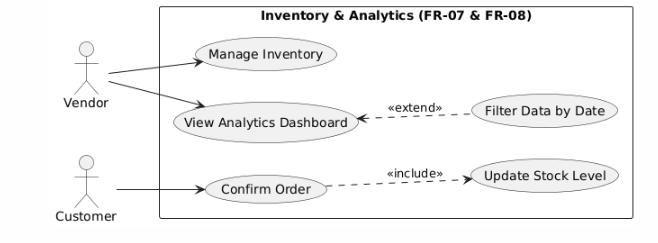
\includegraphics[width=1\linewidth]{figures/dg05.png}
    \caption{Inventory and analytics}
    \label{fig:placeholder}
\end{figure}